\chapter{User-defined functions}
\label{chap:functions}

\section{Defining a function}
\label{func-define}

\app{Gretl} offers a mechanism for defining functions, which may be
called via the command line, in the context of a script, or (if
packaged appropriately, see section~\ref{sec:func-packages}) via the
program's graphical interface.

The syntax for defining a function looks like this:\footnote{The
  syntax given here differs from the standard prior to \app{gretl}
  version 1.8.4.  For reasons of backward compatibility the old syntax
  is still supported; see section~\ref{sec:old-func} for details.}

\begin{raggedright}
\texttt{function} \textsl{return-type} \textsl{function-name}
\texttt{(}\textsl{parameters}\texttt{)} \\
\qquad  \textsl{function body} \\
\texttt{end function}
\end{raggedright}

The opening line of a function definition contains these elements, in
strict order:

\begin{enumerate}
\item The keyword \texttt{function}.
\item \textsl{return-type}, which states the type of value returned by
  the function, if any.  This must be one of \texttt{void} (if the
  function does not return anything), \texttt{scalar},
  \texttt{series}, \texttt{matrix}, \texttt{list} or \texttt{string}.
\item \textsl{function-name}, the unique identifier for the
  function.  Names must start with a letter. They have a maximum
  length of 31 characters; if you type a longer name it will be
  truncated.  Function names cannot contain spaces.  You will get an
  error if you try to define a function having the same name as an
  existing \app{gretl} command.
\item The functions's \textsl{parameters}, in the form of a
  comma-separated list enclosed in parentheses.  This may be run
  into the function name, or separated by white space as shown.
\end{enumerate}

Function parameters can be of any of the types shown
below.\footnote{An additional parameter type is available for GUI use,
  namely \texttt{obs}; this is equivalent to \texttt{int} except for
  the way it is represented in the graphical interface for calling a
  function.}

\begin{center}
\begin{tabular}{ll}
\multicolumn{1}{c}{Type} & 
\multicolumn{1}{c}{Description} \\ [4pt]
\texttt{bool}   & scalar variable acting as a Boolean switch \\
\texttt{int}    & scalar variable acting as an integer  \\
\texttt{scalar} & scalar variable \\
\texttt{series} & data series \\
\texttt{list}   & named list of series \\
\texttt{matrix} & matrix or vector \\
\texttt{string} & string variable or string literal \\
\texttt{bundle} & all-purpose container (see section~\ref{sec:Bundles})
\end{tabular}
\end{center}

Each element in the listing of parameters must include two terms: a
type specifier, and the name by which the parameter shall be known
within the function.  An example follows:
%    
\begin{code}
function scalar myfunc (series y, list xvars, bool verbose)
\end{code}

Each of the type-specifiers, with the exception of \texttt{list} and
\texttt{string}, may be modified by prepending an asterisk to the
associated parameter name, as in
%    
\begin{code}
function scalar myfunc (series *y, scalar *b)
\end{code}

The meaning of this modification is explained below (see section
\ref{funscope}); it is related to the use of pointer arguments in the
C programming language.

\subsection{Function parameters: optional refinements}

Besides the required elements mentioned above, the specification of a
function parameter may include some additional fields, as follows:
\begin{itemize}
\item The \texttt{const} modifier.
\item For \texttt{scalar} or \texttt{int} parameters: minimum, maximum
  and default values; or for \texttt{bool} parameters, just a default
  value.
\item For optional pointer and list arguments (see
  section~\ref{func-details}), the special default value
  \texttt{null}.
\item For all parameters, a descriptive string.
\item For \texttt{int} parameters with minimum and maximum values
  specified, a set of strings to associate with the allowed numerical
  values (value labels).
\end{itemize}

The first two of these options may be useful in many contexts; the
last two may be helpful if a function is to be packaged for use in
the \app{gretl} GUI (but probably not otherwise). We now expand on
each of the options.

\begin{itemize}

\item The \texttt{const} modifier: must be given as a prefix to the
  basic parameter specification, as in
%    
\begin{code}
const matrix M
\end{code} 
%
This constitutes a promise that the corresponding argument will not be
modified within the function; \app{gretl} will flag an error if
the function attempts to modify the argument.

\item Minimum, maximum and default values for \texttt{scalar} or
  \texttt{int} types: These values should directly follow the name of
  the parameter, enclosed in square brackets and with the individual
  elements separated by colons.  For example, suppose we have an
  integer parameter \texttt{order} for which we wish to specify a
  minimum of 1, a maximum of 12, and a default of 4.  We can write
%    
\begin{code}
int order[1:12:4]
\end{code} 
%
If you wish to omit any of the three specifiers, leave the
corresponding field empty.  For example \texttt{[1::4]} would specify
a minimum of 1 and a default of 4 while leaving the maximum
unlimited.  

For a parameter of type \texttt{bool} (whose values are just zero or
non-zero), you can specify a default of 1 (true) or 0 (false), as in
%    
\begin{code}
bool verbose[0]
\end{code} 

\item Descriptive string: This will show up as an aid to the user if
  the function is packaged (see section~\ref{sec:func-packages} below)
  and called via \app{gretl}'s graphical interface.  The string should
  be enclosed in double quotes and separated from the preceding
  elements of the parameter specification with a space, as in
%
\begin{code}
series y "dependent variable"
\end{code} 

\item Value labels: These may be used only with \texttt{int}
  parameters for which minimum and maximum values have been specified,
  so there is a fixed number of admissible values, and the number of
  labels must match the number of values. They will show up in the
  graphical interface in the form of a drop-down list, making the
  function writer's intent clearer when an integer argument represents
  a categorical selection. A set of value labels must be enclosed in
  braces, and the individual labels must be enclosed in double quotes
  and separated by commas or spaces.  For example:
%
\begin{code}
int case[1:3:1] {"Fixed effects", "Between model", "Random effects"}
\end{code} 

\end{itemize}

If two or more of the trailing optional fields are given in a
parameter specification, they must be given in the order shown above:
min--max--default, description, value labels. Note that there is no
facility for ``escaping'' characters within descriptive strings or
value labels; these may contain spaces but they cannot contain the
double-quote character.  

Here is an example of a well-formed function specification using all
the elements mentioned above:
%
\begin{code}
function matrix myfunc (series y "dependent variable",
                        list X "regressors",
                        int p[0::1] "lag order",
                        int c[1:2:1] "criterion" {"AIC", "BIC"},
                        bool quiet[0])
\end{code} 

One advantage of specifying default values for parameters, where
applicable, is that in script or command-line mode users may omit
trailing arguments that have defaults. For example, \texttt{myfunc}
above could be invoked with just two arguments, corresponding to
\texttt{y} and \texttt{X}; implicitly \texttt{p} = 1, \texttt{c} = 1
and \texttt{quiet} is false.

\subsection{Functions taking no parameters}

You may define a function that has no parameters (these are called
``routines'' in some programming languages).  In this case,  
use the keyword \texttt{void} in place of the listing of parameters:
%    
\begin{code}
function matrix myfunc2 (void)
\end{code}


\subsection{The function body}
   
The \textsl{function body} is composed of \app{gretl} commands, or
calls to user-defined functions (that is, function calls may be
nested).  A function may call itself (that is, functions may be
recursive). While the function body may contain function calls, it may
not contain function definitions.  That is, you cannot define a
function inside another function.  For further details, see
section~\ref{func-details}.


\section{Calling a function}
\label{func-call}

A user function is called by typing its name followed by zero or more
arguments enclosed in parentheses.  If there are two or more arguments
these should be separated by commas.  

There are automatic checks in place to ensure that the number of
arguments given in a function call matches the number of parameters,
and that the types of the given arguments match the types specified in
the definition of the function.  An error is flagged if either of
these conditions is violated.  One qualification: allowance is made
for omitting arguments at the end of the list, provided that default
values are specified in the function definition.  To be precise, the
check is that the number of arguments is at least equal to the number
of \textit{required} parameters, and is no greater than the total
number of parameters.

A scalar, series or matrix argument to a function may be given either
as the name of a pre-existing variable or as an expression which
evaluates to a variable of the appropriate type.  Scalar arguments may
also be given as numerical values.  List arguments must be specified
by name.

The following trivial example illustrates a function call that
correctly matches the function definition.
    
\begin{code}
# function definition
function scalar ols_ess(series y, list xvars)
  ols y 0 xvars --quiet
  scalar myess = $ess
  printf "ESS = %g\n", myess
  return myess
end function
# main script
open data4-1
list xlist = 2 3 4
# function call (the return value is ignored here)
ols_ess(price, xlist)
\end{code}

The function call gives two arguments: the first is a data series
specified by name and the second is a named list of regressors.  Note
that while the function offers the variable \verb+myess+ as a return
value, it is ignored by the caller in this instance.  (As a side note
here, if you want a function to calculate some value having to do with
a regression, but are not interested in the full results of the
regression, you may wish to use the \option{quiet} flag with the
estimation command as shown above.)
    
A second example shows how to write a function call that assigns
a return value to a variable in the caller:
    
\begin{code}
# function definition
function series get_uhat(series y, list xvars)
  ols y 0 xvars --quiet
  series uh = $uhat
  return uh
end function
# main script
open data4-1
list xlist = 2 3 4
# function call
series resid = get_uhat(price, xlist)
\end{code}

\section{Deleting a function}
\label{func-del}

If you have defined a function and subsequently wish to clear it out
of memory, you can do so using the keywords \texttt{delete} or
\texttt{clear}, as in

\begin{code}
function myfunc delete
function get_uhat clear
\end{code}

Note, however, that if \texttt{myfunc} is already a defined function,
providing a new definition automatically overwrites the previous one,
so it should rarely be necessary to delete functions explicitly.

\section{Function programming details}
\label{func-details}

\subsection{Variables versus pointers}
\label{funscope}

Series, scalar, and matrix arguments to functions can be passed in two
ways: ``as they are'', or as pointers. For example, consider the
following:
\begin{code}
function series triple1(series x)
  return 3*x
end function
  
function series triple2(series *x)
  return 3*x
end function
\end{code}

These two functions are nearly identical (and yield the same result);
the only difference is that you need to feed a series into
\texttt{triple1}, as in \texttt{triple1(myseries)}, while
\texttt{triple2} must be supplied a \emph{pointer} to a series, as in
\texttt{triple2(\&myseries)}. 

Why make the distinction? There are two main reasons for doing so:
modularity and performance.

By modularity we mean the insulation of a function from the rest of
the script which calls it.  One of the many benefits of this approach
is that your functions are easily reusable in other contexts.  To
achieve modularity, \emph{variables created within a function are
  local to that function, and are destroyed when the function exits},
unless they are made available as return values and these values are
``picked up'' or assigned by the caller.
    
In addition, functions do not have access to variables in ``outer
scope'' (that is, variables that exist in the script from which the
function is called) except insofar as these are explicitly passed to
the function as arguments.

By default, when a variable is passed to a function as an argument,
what the function actually ``gets'' is a \emph{copy} of the outer
variable, which means that the value of the outer variable is not
modified by anything that goes on inside the function.  But the use of
pointers allows a function and its caller to cooperate such that
an outer variable can be modified by the function.  In effect, this
allows a function to ``return'' more than one value (although only one
variable can be returned directly --- see below).  The parameter in
question is marked with a prefix of \texttt{*} in the function
definition, and the corresponding argument is marked with the
complementary prefix \verb+&+ in the caller.  For example,
%
\begin{code}
function series get_uhat_and_ess(series y, list xvars, scalar *ess)
  ols y 0 xvars --quiet
  ess = $ess
  series uh = $uhat
  return uh
end function
# main script
open data4-1
list xlist = 2 3 4
# function call
scalar SSR
series resid = get_uhat_and_ess(price, xlist, &SSR)
\end{code}
%
In the above, we may say that the function is given the \emph{address}
of the scalar variable \texttt{SSR}, and it assigns a value to that
variable (under the local name \texttt{ess}).  (For anyone used to
programming in C: note that it is not necessary, or even possible, to
``dereference'' the variable in question within the function using the
\texttt{*} operator.  Unadorned use of the name of the variable is
sufficient to access the variable in outer scope.)

An ``address'' parameter of this sort can be used as a means of
offering optional information to the caller.  (That is, the
corresponding argument is not strictly needed, but will be used if
present).  In that case the parameter should be given a default value
of \texttt{null} and the the function should test to see if the caller
supplied a corresponding argument or not, using the built-in function
\texttt{isnull()}.  For example, here is the simple function shown
above, modified to make the filling out of the \texttt{ess} value
optional.
%
\begin{code}
function series get_uhat_and_ess(series y, list xvars, scalar *ess[null])
  ols y 0 xvars --quiet
  if !isnull(ess) 
     ess = $ess
  endif
  return $uhat
end function
\end{code}
%
If the caller does not care to get the \texttt{ess} value, it can
use \texttt{null} in place of a real argument:
%
\begin{code}
series resid = get_uhat_and_ess(price, xlist, null)
\end{code}
%
Alternatively, trailing function arguments that have default values 
may be omitted, so the following would also be a valid call:
%
\begin{code}
series resid = get_uhat_and_ess(price, xlist)
\end{code}

Pointer arguments may also be useful for optimizing performance: even if
a variable is not modified inside the function, it may be a good idea
to pass it as a pointer if it occupies a lot of memory. Otherwise, the
time \app{gretl} spends transcribing the value of the variable to the
local copy may be non-negligible, compared to the time the function
spends doing the job it was written for.

Example \ref{ex:perf-pointers} takes this to the extreme.  We define
two functions which return the number of rows of a matrix (a pretty
fast operation).  One function gets a matrix as argument, the other
one a pointer to a matrix.  The two functions are evaluated on a
matrix with 2000 rows and 2000 columns; on a typical system,
floating-point numbers take 8 bytes of memory, so the space occupied
by the matrix is roughly 32 megabytes.

Running the code in example \ref{ex:perf-pointers} will produce output
similar to the following (the actual numbers depend on the
machine you're running the example on):
\begin{code}
Elapsed time: 
	without pointers (copy) = 3.66 seconds,
	with pointers (no copy) = 0.01 seconds.
\end{code}

\begin{script}[htbp]
  \caption{Performance comparison: values versus pointer}
  \label{ex:perf-pointers}
  \begin{scode}
function scalar a(matrix X)
  return rows(X)
end function

function scalar b(const matrix *X)
  return rows(X)
end function

nulldata 10
set echo off
set messages off
X = zeros(2000,2000)
r = 0

set stopwatch
loop 100
  r = a(X)
endloop
fa = $stopwatch

set stopwatch
loop 100
  r = b(&X)
endloop
fb = $stopwatch

printf "Elapsed time:\n\
\twithout pointers (copy) = %g seconds,\n\
\twith pointers (no copy) = %g seconds.\n", fa, fb 
\end{scode}
%$
\end{script}

If a pointer argument is used for this sort of purpose --- and the
object to which the pointer points is not modified by the function ---
it is a good idea to signal this to the user by adding the
\texttt{const} qualifier, as shown for function \texttt{b} in
Example~\ref{ex:perf-pointers}.  When a pointer argument is qualified
in this way, any attempt to modify the object within the function will
generate an error.

One limitation on the use of pointer-type arguments should be noted:
you cannot supply a given variable as a pointer argument more than
once in any given function call. For example, suppose we have a
function that takes two matrix-pointer arguments,
\begin{code}
function scalar pointfunc (matrix *a, matrix *b)
\end{code}
And suppose we have two matrices, \texttt{x} and \texttt{y}, at the
caller level.  The call
\begin{code}
pointfunc(&x, &y)
\end{code}
is OK, but the call
\begin{code}
pointfunc(&x, &x) # will not work
\end{code}
will generate an error.

\subsection{List arguments}

The use of a named list as an argument to a function gives a means of
supplying a function with a set of variables whose number is unknown
when the function is written --- for example, sets of regressors or
instruments.  Within the function, the list can be passed on to
commands such as \texttt{ols}.  

A list argument can also be ``unpacked'' using a \texttt{foreach} loop
construct, but this requires some care.  For example, suppose you have
a list \texttt{X} and want to calculate the standard deviation of each
variable in the list.  You can do:
%
\begin{code}
loop foreach i X
   scalar sd_$i = sd(X.$i)
endloop
\end{code}

\textit{Please note}: a special piece of syntax is needed in this
context.  If we wanted to perform the above task on a list in a
regular script (not inside a function), we could do
%
\begin{code}
loop foreach i X
   scalar sd_$i = sd($i)
endloop
\end{code}
%
where \dollar{i} gets the name of the variable at position $i$ in the
list, and \verb|sd($i)| gets its standard deviation.  But inside a
function, working on a list supplied as an argument, if we want to
reference an individual variable in the list we must use the syntax
\textsl{listname.varname}.  Hence in the example above we write
\verb|sd(X.$i)|.

This is necessary to avoid possible collisions between the name-space
of the function and the name-space of the caller script.  For example,
suppose we have a function that takes a list argument, and that
defines a local variable called \texttt{y}.  Now suppose that this
function is passed a list containing a variable named \texttt{y}.  If
the two name-spaces were not separated either we'd get an error, or
the external variable \texttt{y} would be silently over-written by the
local one.  It is important, therefore, that list-argument variables
should not be ``visible'' by name within functions.  To ``get hold
of'' such variables you need to use the form of identification just
mentioned: the name of the list, followed by a dot, followed by the
name of the variable.

\paragraph{Constancy of list arguments} When a named list of
variables is passed to a function, the function is actually provided
with a copy of the list.  The function may modify this copy (for
instance, adding or removing members), but the original list at the
level of the caller is not modified.

\paragraph{Optional list arguments} If a list argument to a function is
optional, this should be indicated by appending a default value of
\texttt{null}, as in
%
\begin{code}
function scalar myfunc (scalar y, list X[null])
\end{code}
%
In that case, if the caller gives \texttt{null} as the list argument
(or simply omits the last argument) the named list \texttt{X} inside the
function will be empty.  This possibility can be detected using the
\texttt{nelem()} function, which returns 0 for an empty list.

\subsection{String arguments}

String arguments can be used, for example, to provide flexibility in
the naming of variables created within a function.  In the following
example the function \texttt{mavg} returns a list containing two
moving averages constructed from an input series, with the names of
the newly created variables governed by the string argument.
%
\begin{code}
function list mavg (series y, string vname)
   series @vname_2 = (y+y(-1)) / 2
   series @vname_4 = (y+y(-1)+y(-2)+y(-3)) / 4
   list retlist = @vname_2 @vname_4
   return retlist
end function

open data9-9
list malist = mavg(nocars, "nocars")
print malist --byobs
\end{code}
%
The last line of the script will print two variables named
\verb|nocars_2| and \verb|nocars_4|.  For details on the handling of
named strings, see chapter~\ref{chap-persist}.

If a string argument is considered optional, it may be given a
\texttt{null} default value, as in
%
\begin{code}
function scalar foo (series y, string vname[null])
\end{code}

\subsection{Retrieving the names of arguments}

The variables given as arguments to a function are known inside the
function by the names of the corresponding parameters.  For example,
within the function whose signature is
%
\begin{code}
function void somefun (series y)
\end{code}
%
we have the series known as \texttt{y}.  It may be useful, however, to
be able to determine the names of the variables provided as arguments.
This can be done using the function \texttt{argname}, which takes the
name of a function parameter as its single argument and returns a
string.  Here is a simple illustration:
%
\begin{code}
function void namefun (series y)
  printf "the series given as 'y' was named %s\n", argname(y)
end function

open data9-7
namefun(QNC)
\end{code}
%
This produces the output
%
\begin{code}
the series given as 'y' was named QNC
\end{code}

Please note that this will not always work: the arguments given
to functions may be anonymous variables, created on the fly, as in
\texttt{somefun(log(QNC))} or \texttt{somefun(CPI/100)}.  In that case
the \textsf{argname} function fails to return a string.  Function
writers who wish to make use of this facility should check the return
from \texttt{argname} using the \texttt{isstring()} function, which
returns 1 when given the name of a string variable, 0 otherwise.

\subsection{Return values}

Functions can return nothing (just printing a result, perhaps), or
they can return a single variable --- a scalar, series, list, matrix,
string, or bundle (see section~\ref{sec:Bundles}).  The return value,
if any, is specified via a statement within the function body
beginning with the keyword \texttt{return}, followed by either the
name of a variable (which must be of the type announced on the first
line of the function definition) or an expression which produces a
value of the correct type.

Having a function return a list or bundle is a way of permitting the
``return'' of more than one variable.  For example, you can define
several series inside a function and package them as a list; in this
case they are not destroyed when the function exits.  Here is a simple
example, which also illustrates the possibility of setting the
descriptive labels for variables generated in a function.
%    
\begin{code}
function list make_cubes (list xlist)
   list cubes = null
   loop foreach i xlist --quiet
      series $i3 = (xlist.$i)^3
      setinfo $i3 -d "cube of $i"
      list cubes += $i3
   endloop
   return cubes
end function

open data4-1
list xlist = price sqft
list cubelist = make_cubes(xlist)
print xlist cubelist --byobs
labels
\end{code}
%$

A \texttt{return} statement causes the function to return (exit) at
the point where it appears within the body of the function.  A
function may also exit when (a) the end of the function code is
reached (in the case of a function with no return value), (b) a
\app{gretl} error occurs, or (c) a \verb+funcerr+ statement is
reached.

The \verb+funcerr+ keyword, which may be followed by a string enclosed
in double quotes, causes a function to exit with an error flagged.  If
a string is provided, this is printed on exit, otherwise a generic
error message is printed.  This mechanism enables the author of a
function to pre-empt an ordinary execution error and/or offer a more
specific and helpful error message.  For example,
%
\begin{code}
if nelem(xlist) = 0
   funcerr "xlist must not be empty"
endif
\end{code}

A function may contain more than one \texttt{return} statement, as in
%
\begin{code}
function scalar multi (bool s)
   if s
      return 1000
   else
      return 10
   endif
end function
\end{code}
%
However, it is recommended programming practice to have a single
return point from a function unless this is very inconvenient.  The
simple example above would be better written as
%
\begin{code}
function scalar multi (bool s)
   return s ? 1000 : 10
end function
\end{code}
    

\subsection{Error checking}

When gretl first reads and ``compiles'' a function definition there is
minimal error-checking: the only checks are that the function name is
acceptable, and, so far as the body is concerned, that you are not
trying to define a function inside a function (see Section
\ref{func-define}). Otherwise, if the function body contains invalid
commands this will become apparent only when the function is called
and its commands are executed.

\subsection{Debugging}

The usual mechanism whereby \app{gretl} echoes commands and reports on
the creation of new variables is by default suppressed when a function
is being executed.  If you want more verbose output from a particular
function you can use either or both of the following commands within
the function:
%
\begin{code}
set echo on
set messages on
\end{code}

Alternatively, you can achieve this effect for all functions via
the command \texttt{set debug 1}.  Usually when you set the value of a
state variable using the \texttt{set} command, the effect applies only
to the current level of function execution.  For instance, if you do
\texttt{set messages on} within function \texttt{f1}, which in turn
calls function \texttt{f2}, then messages will be printed for
\texttt{f1} but not \texttt{f2}.  The debug variable, however, acts
globally; all functions become verbose regardless of their level.

Further, you can do \texttt{set debug 2}: in addition to command echo
and the printing of messages, this is equivalent to setting
\verb|max_verbose| (which produces verbose output from the BFGS
maximizer) at all levels of function execution.

\section{Function packages}
\label{sec:func-packages}

Since \app{gretl} 1.6.0 there has been a mechanism to package
functions and make them available to other users of \app{gretl}.  Here
is a walk-through of the process.

\subsection{Load a function in memory}

There are several ways to load a function:

\begin{itemize}
\item If you have a script file containing function definitions, open
  that file and run it.
\item Create a script file from scratch.  Include at least one
  function definition, and run the script.
\item Open the GUI console and type a function definition
  interactively.  This method is not particularly recommended; you are
  probably better composing a function non-interactively.
\end{itemize}

For example, suppose you decide to package a function that returns the
percentage change of a time series. Open a script file and type
\begin{code}
function series pc(series y "Series to process")
  return 100 * diff(y)/y(-1)
end function
\end{code}
In this case, we have appended a string to the function argument, as
explained in section \ref{func-define}, so as to make our interface
more informative.  This is not obligatory: if you omit the descriptive
string, \app{gretl} will supply a predefined one.

\begin{figure}[htbp]
  \centering
  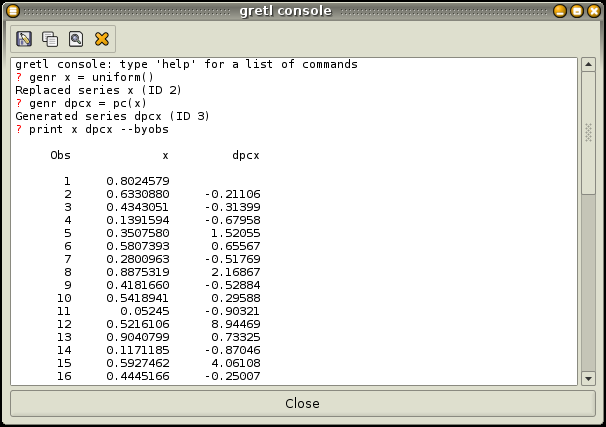
\includegraphics[scale=0.5]{figures/func_check}
  \caption{Output of function check}
  \label{fig:func_check}
\end{figure}

Now run your function. You may want to make sure it works properly by
running a few tests. For example, you may open the console and type

\begin{code}
genr x = uniform()
genr dpcx = pc(x)
print x dpcx --byobs
\end{code}

You should see something similar to figure \ref{fig:func_check}. The
function seems to work ok.  Once your function is debugged, you
may proceed to the next stage.

\subsection{Create a package}

We first present the mechanism for creating a function package via
\app{gretl}'s graphical interface. This can also be done via the
command line, which offers some additional functionality for package
authors; an explanation is given later in this section.

Start the GUI program and take a look at the ``File, Function files'' menu.
This menu contains four items: ``On local machine'', ``On server'', ``Edit
package'', ``New package''.

Select ``New package''.  (This will produce an error message unless at
least one user-defined function is currently loaded in memory --- see
the previous point.)  In the first dialog you get to select:

\begin{itemize}
\item A public function to package.
\item Zero or more ``private'' helper functions.
\end{itemize}

Public functions are directly available to users; private functions are
part of the ``behind the scenes'' mechanism in a function package.

\begin{figure}[htbp]
  \centering
  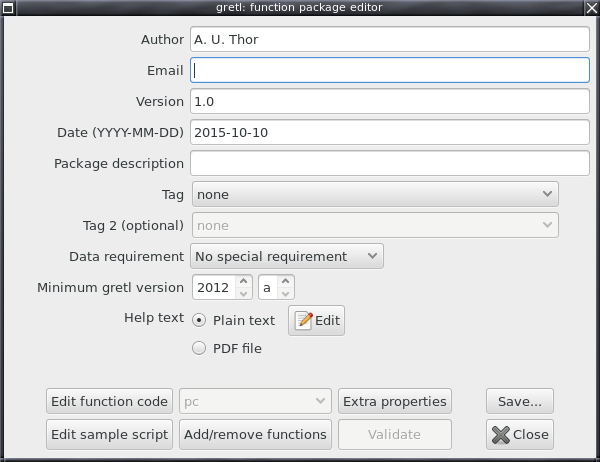
\includegraphics[scale=0.5]{figures/package_editor}
  \caption{The package editor window}
  \label{fig:package_editor}
\end{figure}

On clicking ``OK'' a second dialog should appear (see
Figure~\ref{fig:package_editor}), where you get to enter the package
information (author, version, date, and a short description).  You can
also enter help text for the public interface.  You have a further
chance to edit the code of the function(s) to be packaged, by clicking
on ``Edit function code''.  (If the package contains more than one
function, a drop-down selector will be shown.)  And you get to add a
sample script that exercises your package.  This will be helpful for
potential users, and also for testing.  A sample script is required if
you want to upload the package to the gretl server (for which a
check-box is supplied).

You won't need it right now, but the button labeled ``Save as script''
allows you to ``reverse engineer'' a function package, writing out a
script that contains all the relevant function definitions.

Clicking ``Save'' in this dialog leads you to a File Save dialog.  All
being well, this should be pointing towards a directory named
\texttt{functions}, either under the \app{gretl} system directory (if
you have write permission on that) or the \app{gretl} user directory.
This is the recommended place to save function package files, since
that is where the program will look in the special routine for opening
such files (see below).

Needless to say, the menu command ``File, Function files, Edit package''
allows you to make changes to a local function package.

\vspace{6pt}

A word on the file you just saved.  By default, it will have a
\texttt{.gfn} extension.  This is a ``function package'' file: unlike
an ordinary \app{gretl} script file, it is an XML file containing both
the function code and the extra information entered in the packager.
Hackers might wish to write such a file from scratch rather than using
the GUI packager, but most people are likely to find it awkward.  Note
that XML-special characters in the function code have to be escaped,
e.g.\ \texttt{\&} must be represented as \texttt{\&amp;}.  Also, some
elements of the function syntax differ from the standard script
representation: the parameters and return values (if any) are
represented in XML.  Basically, the function is pre-parsed, and ready
for fast loading using \textsf{libxml}.

\vspace{6pt}

\subsection{Load a package}

Why package functions in this way?  To see what's on offer so far, try
the next phase of the walk-through.

Close gretl, then re-open it.  Now go to ``File, Function files, On
local machine''. If the previous stage above has gone OK, you should
see the file you packaged and saved, with its short description.  If
you click on ``Info'' you get a window with all the information gretl
has gleaned from the function package.  If you click on the ``View
code'' icon in the toolbar of this new window, you get a script view
window showing the actual function code. Now, back to the ``Function
packages'' window, if you click on the package's name, the relevant
functions are loaded into \app{gretl}'s workspace, ready to be called
by clicking on the ``Call'' button.

After loading the function(s) from the package, open the GUI console.
Try typing \texttt{help foo}, replacing \texttt{foo} with the name of
the public interface from the loaded function package: if any help text
was provided for the function, it should be presented.

In a similar way, you can browse and load the function packages
available on the \app{gretl} server, by selecting ``File, Function
files, On server''.

Once your package is installed on your local machine, you can use the
function it contains via the graphical interface as described above,
or by using the CLI, namely in a script or through the console. In the
latter case, you load the function via the \texttt{include} command,
specifying the package file as the argument, complete with the
\texttt{.gfn} extension.

\begin{figure}[htbp]
  \centering
  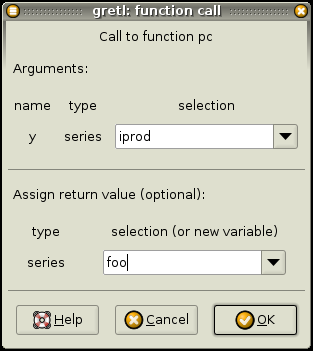
\includegraphics[scale=0.5]{figures/function_call}
  \caption{Using your package}
  \label{fig:function_call}
\end{figure}

To continue with our example, load the file \texttt{np.gdt} (supplied
with \app{gretl} among the sample datasets). Suppose you want to
compute the rate of change for the variable \texttt{iprod} via your
new function and store the result in a series named \texttt{foo}.

Go to ``File, Function files, On local machine''.  You will be shown a
list of the installed packages, including the one you have just
created. If you select it and click on ``Execute'' (or double-click on
the name of the function package), a window similar to the one shown
in figure \ref{fig:function_call} will appear.  Notice that the
description string ``Series to process'', supplied with the function
definition, appears to the left of the top series chooser.

Click ``Ok'' and the series \texttt{foo} will be generated (see figure
\ref{fig:iprod_pc}).  You may have to go to ``Data, Refresh data'' in
order to have your new variable show up in the main window variable
list (or just press the ``r'' key).

\begin{figure}[htbp]
  \centering
  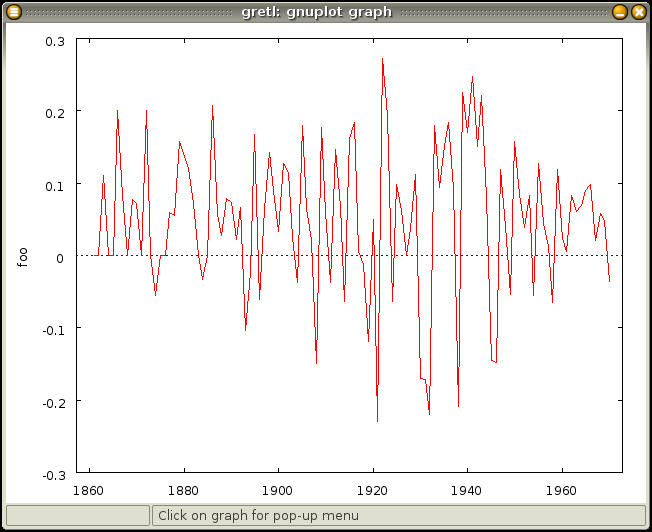
\includegraphics[scale=0.5]{figures/iprod_pc}
  \caption{Percent change in industrial production}
  \label{fig:iprod_pc}
\end{figure}

Alternatively, the same could have been accomplished by the script
\begin{code}
include pc.gfn
open np
foo = pc(iprod)
\end{code}

\subsection{Creating a package via the command line}

The mechanism described above, for creating function packages using
the GUI, is likely to be convenient for small to medium-sized packages
but may be too cumbersome for ambitious packages that include a large
hierarchy of private functions. To facilitate the building of such
packages \app{gretl} offers the \texttt{makepkg} command.

To use \texttt{makepkg} you create three files: a driver script that
loads all the functions you want to package and invokes
\texttt{makepkg}; a small, plain-text specification file that contains
the required package details (author, version, etc.); and (in the
simplest case) a plain text help file.  You run the driver script and
\app{gretl} writes the package (\texttt{.gfn}) file.

We first illustrate with a simple notional package. We have a gretl
script file named \texttt{foo.inp} that contains a function,
\texttt{foo}, that we want to package. Our driver script would then
look like this
%
\begin{code}
include foo.inp
makepkg foo.gfn
\end{code}
%
Note that the \texttt{makepkg} command takes one argument, the name of
the package file to be created. The package \emph{specification file}
should have the same basename but the extension \texttt{.spec}. In
this case \app{gretl} will therefore look for \texttt{foo.spec}. It
should look something like this:
%
\begin{code}
# foo.spec
author = A. U. Thor
version = 1.0
date = 2011-02-01
description = Does something with time series
public = foo 
help = foohelp.txt
sample-script = example.inp
min-version = 1.9.3
data-requirement = needs-time-series-data
\end{code}

As you can see, the format of each line in this file is \texttt{key =
  value}, with two qualifications: blank lines are permitted (and
ignored, as are comment lines that start with \verb|#|). 

All the fields included in the above example are required, with the
exception of \texttt{data-requirement}, though the order in which they
appear is immaterial. Here's a run-down of the basic fields:

\begin{itemize}
\item \texttt{author}: the name(s) of the author(s). Accented or other
  non-ASCII characters should be given as UTF-8.
\item \texttt{version}: the version number of the package, which should
  be limited to two integers separated by a period.
\item \texttt{date}: the release date of the current verson of the
  package, in ISO 8601 format: YYYY-MM-DD.
\item \texttt{description}: a brief description of the functionality
  offered by the package. This will be displayed in the GUI function
  packages window so it should be just one short line.
\item \texttt{public}: the listing of public functions.
\item \texttt{help}: the name of a plain text (UTF-8) file containing
  help; all packages must provide help.
\item \texttt{sample-script}: the name of a sample script that
 illustrates use of the package; all packages must supply a
 sample script.
\item \texttt{min-version}: the minimum version of gretl required
 for the package to work correctly. If you're unsure about this,
 the conservative thing is to give the current \app{gretl} version.
\end{itemize}

The \texttt{public} field indicates which function or functions are to
be made directly available to users (as opposed to private ``helper''
functions).  In the example above there is just one public
function. Note that any functions in memory when \texttt{makepkg} is
invoked, other than those designated as public, are assumed to be
private functions that should also be included in the package. That
is, the list of private functions (if any) is implicit.

The \texttt{data-requirement} field should be specified if the package
requires time-series or panel data, or alternatively if no dataset is
required.  If the \texttt{data-requirement} field is omitted, the
assumption is that the package needs a dataset in place, but it
doesn't matter what kind; if the packaged functions do not use any
series or lists this requirement can be explicitly relaxed.  Valid
values for this field are:

\begin{center}
\begin{tabular}{ll}
\texttt{needs-time-series-data} & (any time-series data OK) \\ 
\texttt{needs-qm-data} & (must be quarterly or monthly) \\ 
\texttt{needs-panel-data} & (must be a panel) \\
\texttt{no-data-ok} & (no dataset is needed) \\
\end{tabular}
\end{center}

For a more complex example, let's look at the \app{gig}
(GARCH-in-gretl) package.  The driver script for building \app{gig}
looks something like this:
%
\begin{code}
set echo off
set messages off
include gig_mle.inp
include gig_setup.inp
include gig_estimate.inp
include gig_printout.inp
include gig_plot.inp
makepkg gig.gfn
\end{code}

In this case the functions to be packaged (of which there are many)
are distributed across several script files, each of which is the
target of an \texttt{include} command.  The \texttt{set} commands at
the top are included to cut down on the verbosity of the output.

The content of \texttt{gig.spec} is as follows:
%
\begin{code}
author = Riccardo "Jack" Lucchetti and Stefano Balietti
version = 2.0
date = 2010-12-21
description = An assortment of univariate GARCH models
public = GUI_gig \
    gig_setup gig_set_dist gig_set_pq gig_set_vQR \
    gig_print gig_estimate \
    gig_plot gig_dplot \
    gig_bundle_print GUI_gig_plot

gui-main = GUI_gig
bundle-print = gig_bundle_print
bundle-plot = GUI_gig_plot
help = gig.pdf
sample-script = examples/example1.inp
min-version = 1.9.3
data-requirement = needs-time-series-data
\end{code}

Note that backslash continuation can be used for the elements of the
\texttt{public} function listing.

In addition to the fields shown in the simple example above,
\texttt{gig.spec} includes three optional fields: \texttt{gui-main},
\texttt{bundle-print} and \texttt{bundle-plot}. These keywords are
used to designate certain functions as playing a special role in the
\app{gretl} graphical interface. A function picked out in this way
must be in the \texttt{public} list and must satisfy certain
further requirements.  
%
\begin{itemize}
\item \texttt{gui-main}: this specifies a function as the one which
  will be presented automatically to GUI users (instead of users'
  being faced with a choice of interfaces). This makes sense only for
  packages that have multiple public functions. In addition, the
  \texttt{gui-main} function must return a \texttt{bundle} (see
  section~\ref{sec:Bundles}).
\item \texttt{bundle-print}: this picks out a function that should be
  used to print the contents of a bundle returned by the
  \texttt{gui-main} function. It must take a pointer-to-bundle as its
  first argument. The second argument, if present, should be an
  \texttt{int} switch, with two or more valid values, that controls the
  printing in some way. Any further arguments must have default values
  specified so that they can be omitted.
\item \texttt{bundle-plot}: selects a function for the role of
  producing a plot or graph based on the contents of a returned
  bundle. The requirements on this function are as for 
  \texttt{bundle-print}.
\end{itemize}

The ``GUI special'' tags support a user-friendly mode of operation.
On a successful call to \texttt{gui-main}, \app{gretl} opens a 
window displaying the contents of the returned bundle (formatted
via \texttt{bundle-print}). Menus in this window give the user the
option of saving the entire bundle (in which case it's represented
as an icon in the ``icon view'' window) or of extracting specific
elements from the bundle (series or matrices, for example). 

If the package has a \texttt{bundle-plot} function, the bundle window
also has a \textsf{Graph} menu. In \app{gig}, for example, the
\texttt{bundle-plot} function has this signature:
%
\begin{code}
function void GUI_gig_plot(bundle *model, int ptype[0:1:0] \
                           "Plot type" {"Time series", "Density"})
\end{code}

The \texttt{ptype} switch is used to choose between a time-series plot
of the residual and its conditional variance, and a kernel density
plot of the innovation against the theoretical distribution it is
supposed to follow. The use of the value-labels \texttt{Time series}
and \texttt{Density} means that the \textsf{Graph} menu will display
these two choices.

One other feature of the \app{gig} spec file is noteworthy: the
\texttt{help} field specifies \texttt{gig.pdf}, documentation in PDF
format. Unlike plain-text help, this cannot be rolled into the
\texttt{gfn} (XML) file produced by the \texttt{makepkg} command;
rather, both \texttt{gig.gfn} and \texttt{gig.pdf} are packaged into a
zip archive for distribution. This represents a form of package
which is new in \app{gretl} 1.9.4. More details will be made
available before long. 

\section{Memo: updating old-style functions}
\label{sec:old-func}

As mentioned at the start of this chapter, different rules were in
force for defining functions prior to \app{gretl} 1.8.4. While the old
syntax is still supported to date, this may not always be the
case. But it is straightforward to convert a function to the new
style. The only thing that must be changed for compatibility with the
new syntax is the declaration of the function's return
type. Previously this was placed inline in the \texttt{return}
statement, whereas now it is placed right after the \texttt{function}
keyword. For example:
%
\begin{code}
# old style
function triple (series x)
  y = 3*x
  return series y # note the "series" here
end function

# new style
function series triple (series x)
  y = 3*x
  return y
end function
\end{code}

Note also that the role of the \texttt{return} statement has changed
(and its use has become more flexible):

\begin{itemize}
\item The \texttt{return} statement now causes the function to return
  directly, and you can have more than one such statement, wrapped in
  conditionals. Before there could only be one \texttt{return}
  statement, and its role was just to specify the type available for
  assignment by the caller.
\item The final element in the \texttt{return} statement can now be an
  expression that evaluates to a value of the advertised return type;
  before, it had to be the name of a pre-defined variable.
\end{itemize}


%%% Local Variables: 
%%% mode: latex
%%% TeX-master: "gretl-guide"
%%% End: 

